\section{Marco teórico}

\subsection{Ciclo de carga}

%Carga en dos o tres etapas según la tensión de la batería en el momento de su conexión: precarga, corriente constante y tensión constante. 
Está dividido en dos o tres etapas según la tensión de la batería en el momento de su conexión: precarga, corriente constante y tensión constante \cite{icr18650s3}\cite{ncr18650ga}.

La etapa de precarga sólo tiene lugar en baterías que han sido profundamente descargadas y cuya tensión sea superior a 22V e inferior a 30V.
Se le entrega una corriente constante, cuyo valor se limita a un quinto de la corriente de carga nominal.

Una vez que la batería supera la tensión de 30V, la carga continúa con la etapa de corriente constante hasta llegar a una tensión de 42V.
Su intensidad depende del modo seleccionado en un rango discreto: 1A, 1.6A, 2.1A, 3.2A, 4.3A, 5A, 6.7A.

En la etapa final de tensión constante, se mantiene la tensión de salida en 42V mientras la corriente disminuye hasta un décimo de la corriente nominal de carga,
momento en el cual se produce el corte ya que la batería se encuentra completamente cargada. 

\begin{figure}[H]
    \centering
    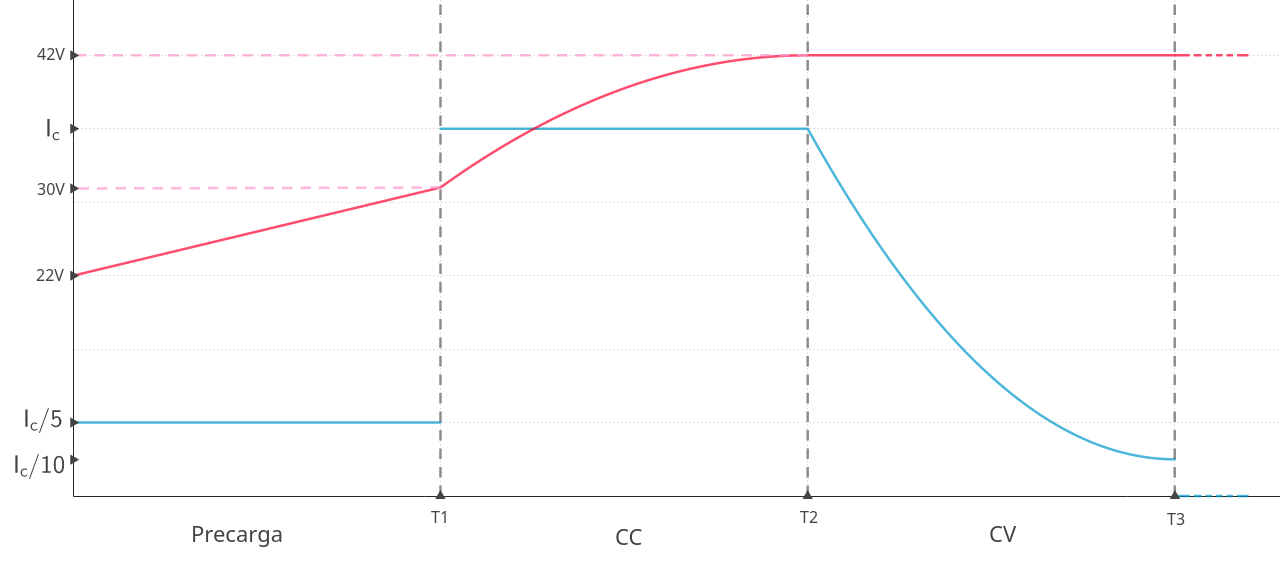
\includegraphics[width=0.8\textwidth]{images/perfil_de_carga.png}
    \caption{Perfil de carga}
    \label{fig:perfil_de_carga}
\end{figure}

\subsection{Sistema de gestión de baterías (BMS)}

Un Sistema de Gestión de Baterías o Battery Management System (BMS) es un sistema electrónico que gestiona y controla baterías recargables,
garantizando su protección a partir de la limitación de su funcionamiento dentro del área de operación segura.
Realiza un seguimiento de su estado, recopila, procesa y almacena los datos obtenidos en tiempo real, controla su entorno y puede intercambiar información con dispositivos externos.
Su función principal es el balance o equilibrio de las celdas de la batería \cite{bms}.

\subsubsection{Funciones}

\paragraph{Medición de parámetros}
Garantiza que la carga y la descarga no excedan las recomendaciones del fabricante y permite saber en qué momento apagar la batería por bajo voltaje. 

\begin{itemize}
    \item Temperatura ambiente y de las celdas de la batería
    \item Intensidad de corriente en la entrada y la salida
    \item Tensión de cada celda
\end{itemize}

\paragraph{Protección}
El sistema genera alarmas tempranas y corta el suministro del cargador en caso de falla o condiciones de funcionamiento inseguras tales como:

\begin{itemize}
    \item Sobre cargas: Evita que la batería supere el valor máximo de tensión especificado por el fabricante durante la carga de la batería.
    \item Sobre descargas: Evita que la batería continúe alimentando a la carga cuando la misma posee muy baja tensión y garantizar futuras cargas. 
    \item Sobre corrientes: Ocasionadas por una sobrecarga, un cortocircuito o una falla a tierra.
    \item Temperaturas extremas: Ocasionadas ante fallos en las celdas o por sobrecalentamiento.
\end{itemize}

\paragraph{Balanceo}
Usualmente las baterías están conformadas por celdas que no tienen exactamente la misma capacidad. 
Para compensar este desbalance, se requiere de un balanceo que equilibre las tensiones de todas las celdas. 
Dependiendo de la química de la batería, cada una de ellas tiene un rango de tensión ligeramente diferente donde debe ocurrir la carga o descarga, pero en todos los casos el uso de baterías fuera de este rango puede reducir su ciclo de vida. 
Por ejemplo, las celdas frías deben cargarse a una tensión superior y las celdas en mal estado pueden evitar que otras se carguen por completo. 
Por todos estos motivos, las celdas se cargan de forma independiente mediante la conmutación de transistores que permiten el intercambio de energía. Esto maximiza la capacidad y aumenta la vida útil de la batería. También evita grandes sometimientos en comparación a una única celda equivalente dividiendo por igual la tensión de descarga en todas las celdas.

Existen dos tipos de balanceo, los cuales pueden verse ilustrados en la figura \ref{fig:bms-load-balancing}:

\begin{itemize}
    \item Balanceo pasivo: se disipa la energía de las baterías con mayor tensión para igualarlas a las más bajas. Implica un mayor consumo de energía.
    \item Balanceo activo: redistribuye la energía de las celdas con mayor tensión hacia las de menor tensión. Implica un mayor costo de implementación.
\end{itemize}

\begin{figure}[H]
    \centering
    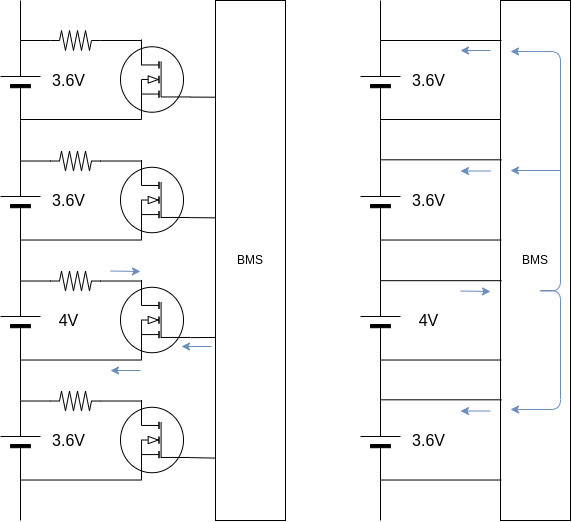
\includegraphics[width=0.7\textwidth]{images/bms-load-balancing.png}
    \caption{Tipos de balanceo de carga. A la izquierda, balanceo pasivo. A la derecha, balanceo activo}
    \label{fig:bms-load-balancing}
\end{figure}

\paragraph{Gestión térmica}
Mantiene a la batería en el rango de operación segura de -10°C hasta 80-85°C, evitando una fuga térmica cuando la temperatura está fuera del rango.  La necesidad de disipar el calor producido por las celdas debido a reacciones electroquímicas es más relevante cuando muchas celdas están agrupadas. En este caso puede utilizarse un sistema de refrigeración activo, como la ventilación forzada.

\paragraph{Evaluación}
Calcula y estima ciertos parámetros relacionados con el estado de la batería.

\begin{itemize}
    \item Estado de carga (SOC)

    Indica la cantidad de energía almacenada utilizable. Permite determinar la carga y descarga óptima y limitar la ventana de operación.

    \item Capacidad

    La capacidad de la batería varía con el tiempo y es el indicador del estado de salud de la celda. Cuando la capacidad se reduce por debajo de cierto límite, la batería llega al fin de su vida útil. Se obtiene descargando la batería en su totalidad a partir de una carga completa.

    $$ Capacidad[Ah] = Intensidad[A] \cdot Tiempo[h] $$

    Existen varios métodos de obtener el SOC como por ejemplo con la tensión de circuito abierto, el conteo de Coulombs, filtros de Kalman, entre otros.

    \item Estado de salud (SOH)

    Se obtiene en base a la capacidad original de la batería y la última capacidad obtenida. La estimación de los parámetros SOC y SOH requieren precisión en los sensores y el desarrollo de complejos algoritmos de estimación.

    \item Tiempo de recarga

    Se estima conociendo la última capacidad obtenida y suponiendo una intensidad de carga constante.

    \item Resistencia interna
    
    Se utiliza para conocer la salud de la batería. Un valor fuera del rango especificado por el fabricante indica que una o varias de las celdas están en mal estado y requieren un reemplazo.
\end{itemize}

\paragraph{Comunicación}
Dependiendo del objetivo del BMS y su construcción, el puerto de comunicación puede ser unidireccional donde los datos a transferir son simples, como la energía restante del sistema, o bidireccional en sistemas más complejos como los buses estandarizados para vehículos eléctricos CAN, RS232, Ethernet, USB, etc. El puerto que soporta el BMS determina la compatibilidad con el resto de las interfaces comunicativas del sistema.

Si bien un BMS incrementa el consumo, costo y la complejidad del sistema, su inclusión es fundamental debido a las numerosas ventajas que presenta:

\begin{itemize}
    \item Descarga uniforme y carga independiente de las celdas en base a su estado.
    \item Permite la operación en su zona segura, estableciendo límites de corriente, tensión y temperatura sobre los cuales se puede esperar que funcione de forma correcta.
    \item Protege la batería mediante desconexión automática en caso de sobre cargas, sobre descargas, sobre corrientes y temperaturas extremas.
    \item Conocer el estado de carga, salud y capacidad de la batería.
    \item Extiende la vida útil de la batería.
    \item Advertencia sobre celdas en mal estado.
    \item Reducción del mantenimiento de la batería.
\end{itemize}

\subsection{Rectificador de entrada AC-DC}

Los circuitos rectificadores AC-DC convierten una tensión alterna en una tensión continua.
Esta etapa es necesaria para poder alimentar con una tensión continua al convertidor DC-DC. \cite{hart_espanol}

\subsubsection{Rectificador de media onda u onda completa}

Si bien el rectificador de media onda es uno de los circuitos más simples al contar únicamente con un diodo,
existen muchas ventajas del rectificador de onda completa frente al de media onda.
La primera de ellas es que la corriente media del generador de alterna es nula, lo cual beneficia a los transformadores. 
La segunda se basa en el hecho de que para una misma carga,
la tensión de rizado pico a pico para el rectificador de onda completa es
aproximadamente la mitad que para el rectificador de media onda. 
Esto se debe a que en el circuito de onda completa,
el tiempo durante el cual se descarga el capacitor es menor que en el circuito de media onda % Pero acá ya estamos hablando de un filtro
en base a la onda sinusoidal rectificada de la segunda mitad de cada período. 
Por todos estos motivos se decidió implementar un rectificador de onda completa.

\subsubsection{Rectificador de onda completa en puente o con toma media}

El rectificador en puente presenta una caída de tensión de 2 diodos entre el generador y la carga. 
La tensión máxima en un diodo polarizado en inversa es el valor pico del generador.
Suelen incluirse en pequeños circuitos integrados. 

La variante con transformador de toma media sólo presenta la caída de tensión de un diodo entre el generador y la carga.
El transformador proporciona aislamiento eléctrico entre el generador y la carga. 
Para una misma potencia entregada por el generador,
los diodos consumen potencia y disminuyen la corriente y potencia que absorbe la carga. 
La tensión máxima en un diodo polarizado en inversa es el doble del valor pico del generador. 
Presenta un mayor tamaño debido a la presencia del transformador que opera en baja frecuencia. 

Como la reducción de tensión a la salida no es significativa en esta aplicación,
con el objetivo de disminuir el tamaño del circuito se decidió utilizar un rectificador de onda completa tipo puente.

\subsubsection{Rectificación controlada}

La rectificación controlada utiliza tiristores para controlar la tensión de salida mediante la modificación del ángulo de conmutación de los mismos.
Los tiristores son interruptores electrónicos controlados que son activados por una señal externa. 
Poseen 3 terminales: ánodo, cátodo y puerta. Presentan altos valores nominales de corriente y tensión.
Soportan altas corrientes y altas tensiones de bloqueo. 

Un ejemplo de tiristores son los rectificadores controlados de silicio (SCR).
Para que conduzcan se los debe polarizar en directa y deben recibir una corriente de puerta. 
Al entrar en conducción no es necesaria la señal de puerta para mantener la corriente de ánodo. 
El SCR continuará conduciendo siempre que la corriente de ánodo sea positiva y esté por arriba de un valor mínimo. 
Mediante conmutadores controlados como los SCR se controla la tensión de salida en un rango limitado de variación, ajustando el ángulo de disparo de cada SCR. 
El ángulo de disparo es el intervalo angular entre la polarización directa del SCR y la aplicación de la señal de puerta. 
Si el ángulo de disparo es 0, el comportamiento es igual al de un rectificador no controlado con diodos. 

Se decidió utilizar rectificación no controlada ya que no se necesita una tensión específica a la salida
y el costo de complejizar el diseño con el agregado de SCRs y un circuito dedicado de disparo no aporta ningún beneficio significativo.

\subsubsection{Filtrado}

Un filtro pasa bajos compuesto por una red LC permite disminuir el rizado,
es decir, la componente de alterna de la señal rectificada. 
Como resultado se logra una tensión de salida aproximadamente continua.
El capacitor mantiene la tensión de salida en un nivel constante y
la bobina suaviza la corriente del rectificador y reduce la corriente de pico en los diodos. 

Para disminuir el número de componentes se decidió utilizar únicamente
un capacitor, cuya capacidad sea la suficiente para obtener una tensión continua.

\subsection{Fuentes de alimentación}

Las fuentes de alimentación otorgan una alta densidad de potencia en un tamaño mediano y con un peso reducido.  
Permiten aislar eléctricamente a la carga de la red de alimentación con una alta eficiencia de conversión.  
En base a la tensión de salida requerida existen fuentes de alimentación AC y DC \cite{rashid}.
Dado el requisito de tensión de salida continua, se debe diseñar una fuente de alimentación DC, las cuales se clasifican en:

\paragraph{Conmutadas}
Tienen una alta eficiencia y pueden suministrar altas corrientes de carga a una tensión baja.
Las topologías más comunes son: fly-back, forward, push–pull, half-bridge y full-bridge.
Por lo general se utilizan 2 etapas de conversión: DC-AC mediante modulación de ancho de pulso (PWM) y AC-DC.
La salida del transformador de potencia, que varía mediante una señal PWM, se convierte en una tensión continua mediante un rectificador de diodos. 
Debido a que el transformador puede operar a una frecuencia muy alta, las fluctuaciones en la tensión de salida se pueden filtrar fácilmente.

\paragraph{Resonantes}
Si la variación de la tensión de salida no es amplia se pueden utilizar inversores de pulso resonante. 
La frecuencia del inversor, que podría ser la misma que la frecuencia de resonancia, es muy alta y la tensión de salida del inversor es casi sinusoidal.
Debido a la oscilación resonante, el núcleo del transformador siempre se restablece y no hay problemas de saturación. 
Los tamaños del transformador y del filtro de salida se reducen debido a la alta frecuencia del inversor.

\paragraph{Bidireccionales}
Aptas para carga y descarga de baterías donde el flujo de potencia es bidireccional.
Este último depende de la tensión de entrada, de la tensión de salida y de la relación de vueltas del transformador. 
Permiten que la corriente inductiva fluya en cualquier dirección y que el flujo de corriente se vuelva continuo.
Requiere sintetizar las funciones de conmutación para obtener las formas de onda de salida deseadas.\\

Dado que no se requiere de un flujo de potencia bidireccional durante la carga de las baterías y la mayor complejidad de las fuentes resonantes, 
se optó por desarrollar una fuente de alimentación conmutada. 

\subsection{Elección del convertidor}

Para seleccionar el convertidor apropiado es necesario analizar los requisitos de la aplicación y las ventajas y desventajas de cada topología.  
Sólo se describe de forma completa la topología utilizada en el proyecto. En cuanto a las restantes, se detallarán los motivos que llevaron a sus exclusiones.  

El convertidor introduce aislación a partir de un transformador de alta frecuencia,
el cual disminuyen el coste, tamaño y peso respecto a uno de baja frecuencia en base al núcleo magnético necesario.
Como se requiere una única tensión de salida no se utilizan múltiples devanados.

Aunque la mayor parte de los convertidores se pueden utilizar para cumplir con los requerimientos de salida, 
los valores nominales del dispositivo de conmutación y el tamaño del transformador limitan sus aplicaciones a una potencia de salida específica. 
Por lo tanto, la elección del convertidor depende del requisito de potencia de salida y de la complejidad que se desea afrontar.
Para el cargador de baterías, el convertidor debe alcanzar una potencia máxima de 300W y debe ser lo más sencillo posible para evitar un costo elevado \cite{hart}.

La topología flyback es la más sencilla al estar integrada por muy pocos componentes. 
La energía se almacena en el primario cuando el conmutador está cerrado y se transfiere a la carga cuando está abierto.
Como desventajas, el tamaño del núcleo del transformador se incrementa con la potencia requerida y en bornes del
interruptor presenta una tensión igual al doble de la tensión máxima de entrada.
En aplicaciones típicas se alcanzan potencias de hasta 150W.

La topología forward con un solo switch disminuye el tamaño del núcleo ya que la energía no necesita almacenarse en el primario.
En esta topología, la energía del generador se transfiere a la carga cuando el interruptor está cerrado.
Como desventajas, al igual que la flyback presenta alta tensión en bornes del interruptor y se eleva el costo debido al agregado de la bobina de filtrado.
La topología forward con dos switches reduce la tensión en bornes del interruptor a la mitad respecto a la de un solo switch (y con ello la disipación de potencia por switch), 
pero el circuito de excitación de uno de los transistores queda flotante respecto a masa. 
La topología con un solo switch admite una potencia de salida entre 150-250W y con 2 switches se eleva a 500W. 
Por lo tanto, en base a los criterios definidos inicialmente se eligió al convertidor forward con dos switches como topología de conversión DC-DC. 

\subsubsection{Convertidor Forward}

Es un convertidor acoplado magnéticamente. El transistor funciona como interruptor, estará cerrado un tiempo $DT$ y abierto el resto del tiempo,
$(1 - D)T$, siendo $T$ el período de conmutación. 
En la figura \ref{fig:conversor_forward} se muestra el esquema del convertidor con un solo switch.
El transformador posee tres devanados: los devanados 1 y 2 transfieren la energía de la
fuente a la carga cuando el interruptor está cerrado; el devanado 3 se usa para proporcionar un
camino a la corriente magnetizante cuando el interruptor está abierto y permite reducirla a cero antes del
inicio de cada período de conmutación. De esta forma se reestablece el núcleo ya que la energía almacenada en el mismo es devuelta a la fuente de entrada del convertidor.
El transformador se modela como tres devanados ideales con una inductancia magnetizante $L_m$ conectada en paralelo con el devanado 1. 
En este modelo simplificado no se incluyen las pérdidas ni las inductancias de dispersión.
En el convertidor forward, $L_m$ es un parámetro no incluido en la relación entrada-salida y se suele adoptar un valor grande.
Además, sólo se opera en el modo de conducción continua por la mayor dificultad del control en base al doble polo existente en el filtro de salida. 

\begin{figure}[ht]
    \centering
    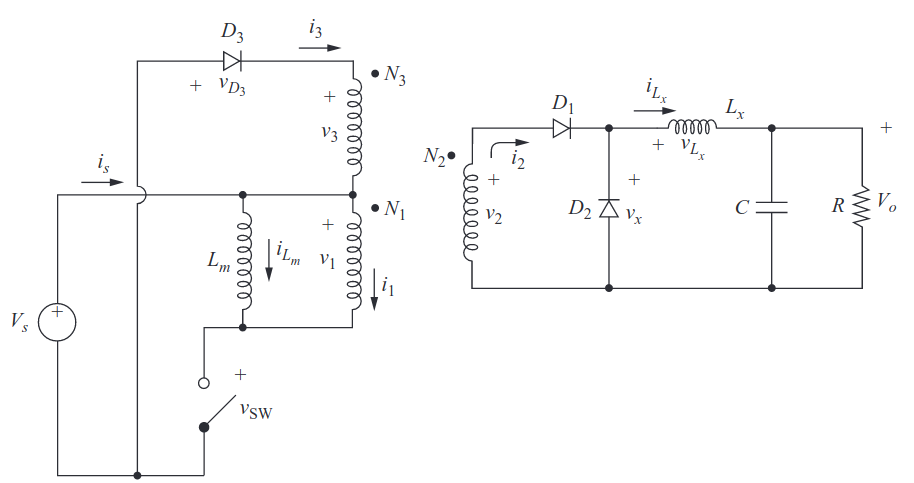
\includegraphics[width=0.8\textwidth]{../images/hart/conversor_forward.png}
    \caption{Esquema del convertidor forward de un solo switch}
    \label{fig:conversor_forward}
\end{figure}

% REVISAR NOMENCLATURA EN BASE A LAS IMÁGENES A UTILIZAR DE LOS LIBROS
Asumiendo modo de conducción continua, operación en estado estacionario, ripple de salida nulo 
y que la corriente en la inductancia del filtro de salida $L_x$ es permanente, existen 2 modos de operación del transistor:

% RASHID EN INGLÉS

\paragraph{Cuando el transistor se encuentra encendido}

En la figura \ref{fig:forward_switch_closed} se muestra el circuito equivalente cuando el interruptor
está cerrado. Al cerrarse el interruptor se establece una tensión en el primer devanado del transformador,
lo cual induce tensiones en el segundo y tercer devanado:

% HART INGLÉS PÁGINA 279 DEL LIBRO 
$$ v_1=V_s $$
$$ v_2=v_1\left(\frac{N_2}{N_1}\right)=V_s\left(\frac{N_2}{N_1}\right) $$
$$ v_3=v_1\left(\frac{N_3}{N_1}\right)=V_s\left(\frac{N_3}{N_1}\right) $$

\begin{figure}[ht]
    \centering
    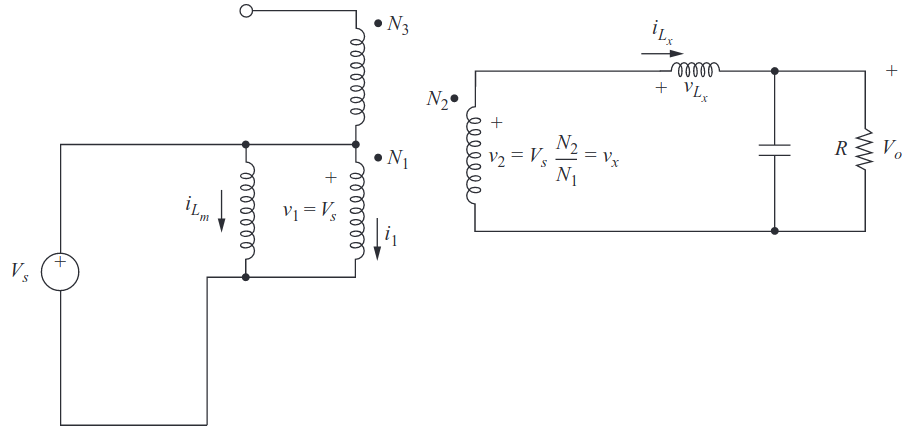
\includegraphics[width=0.8\textwidth]{../images/hart/forward_switch_closed.png}
    \caption{Convertidor forward cuando el interruptor está cerrado}
    \label{fig:forward_switch_closed}
\end{figure}

La tensión $v_2$ positiva polariza en directa a $D_1$ y en reversa a $D_2$. El diodo $D_3$ no conduce ya que su tensión es negativa:

$$ V_{D_3}=-V_s-v_3<0 $$

La tensión en la bobina es:
% vlx
$$ v_{L_x}=v_2-V_0=V_s\left(\frac{N_2}{N_1}\right)-V_o=L_x\frac{di_{L_x}}{dt} $$

Reorganizando los términos obtenemos:

$$ \frac{di_{L_x}}{dt}=\frac{V_s(N_2/N_1)-V_o}{L_x}=\frac{\Delta i_{L_x}}{\Delta t}=\frac{\Delta i_{L_x}}{DT} $$

Como la derivada de la corriente es una constante positiva, la corriente en el inductor aumenta linealmente con el tiempo. 
La variación de corriente cuando el interruptor está cerrado se calcula modificando la ecuación anterior:

$$ (\Delta i_{L_x})_{cerrado}=\left[V_s\left(\frac{N_2}{N_1}\right)-V_o\right]\frac{DT}{L_x} $$

La tensión en la inductancia magnetizante es igual a la tensión en el primario del transformador, por lo cual:

$$ \Delta i_{L_m}=\frac{V_sDT}{L_m} $$

La corriente que circula por el primario comienza a incrementarse,
se transfiere energía del primario al secundario y de aquí al filtro de salida y la carga por medio del diodo $D_1$ polarizado en directa. 
Debido a esta corriente se induce una corriente en el secundario dada por:

$$ i_2=\frac{N_1}{N_2}i_{1} $$

La corriente magnetizante se incrementa linealmente con el tiempo:

$$ i_{mag}=\frac{V_s}{L_m}t $$

La corriente de colector que circula por el transistor es la corriente 
que circula físicamente por el primario y está compuesta por:

$$ i_1'=i_1+i_{mag}=\frac{N_2}{N_1}i_{2}+\frac{V_s}{L_m}t $$

Cuando finaliza el tiempo de conducción del transistor en un tiempo $t=DT$, esta corriente llega a un valor máximo dado por:

$$ I_{1_{max}}'=I_{1_{max}}+\frac{V_sDT}{L_m}=\frac{N_1}{N_2}I_{L_{x_{max}}} +\frac{V_sDT}{L_m} $$

donde $I_{x_{max}}$ es la corriente pico reflejada del secundario en el inductor $L_x$.

La corriente por el inductor también tendrá su valor máximo en $t=DT$:

$$ I_{L_{x_{max}}}=I_{L_x}(0)+\frac{\left[V_s(N_2/N_1)-V_o\right]DT}{L_x} $$

\paragraph{Cuando el transistor se encuentra apagado}
En la figura \ref{fig:forward_switch_open} se muestra el circuito equivalente cuando el interruptor está abierto.  
La corriente magnetizante y la corriente en el inductor del filtro de salida no pueden cambiar instantáneamente cuando el transistor se apaga. 
La continuidad de $i_{L_m}$ establece $ i_1=-i_{L_m} $.
% SACAR DEL TEXTO INICIAL

\begin{figure}[ht]
    \centering
    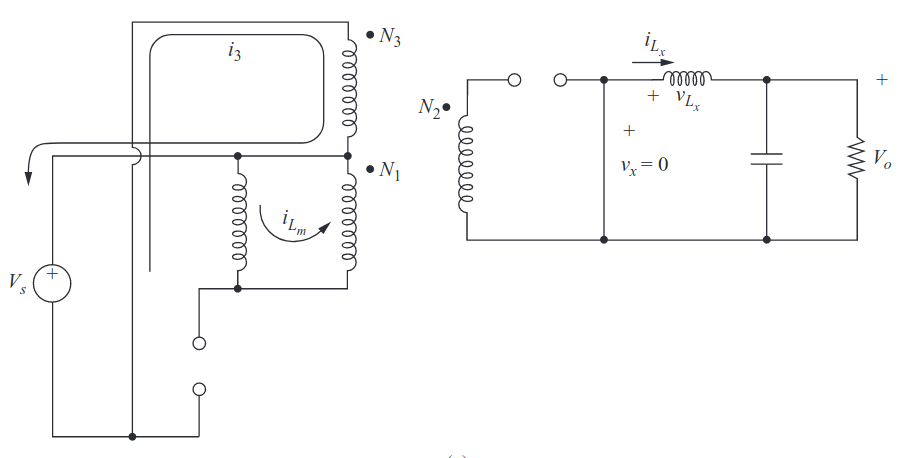
\includegraphics[width=0.8\textwidth]{images/hart/forward_switch_open.png}
    \caption{Convertidor forward cuando el interruptor está abierto}
    \label{fig:forward_switch_open}
\end{figure}

La corriente que sale del terminal con punto homólogo del primer bobinado quiere establecer una corriente que ingresa al terminal 
con punto homólogo del segundo bobinado, pero el diodo $D_1$ no permite la circulación de la corriente en esa dirección. 
Además, la corriente que sale del terminal con punto homólogo del primer bobinado induce una corriente que ingresa al terminal 
con punto homólogo del tercer bobinado. Esto polariza en directa al diodo $D_3$, a la vez que 
se le provee a la corriente magnetizante de un camino a través del tercer bobinado de regreso a la fuente de entrada. 

Con $D_3$ encendido, la tensión en el tercer bobinado resulta:
% HART EN INGLES PÁGINA 280 DEL LIBRO 
$$ v_3=-V_s $$

Esto induce las siguientes tensiones en los otros bobinados:
% ECUACIÓN 7.25
$$ v_1=v_3\left(\frac{N_1}{N_3}\right)=-V_s\left(\frac{N_1}{N_3}\right) $$
$$ v_2=v_3\left(\frac{N_2}{N_3}\right)=-V_s\left(\frac{N_2}{N_3}\right) $$

Con $D_1$ apagado y corriente positiva en el inductor de salida, $D_2$ se polariza en directa. 
Mientras conduce $D_2$, la energía es entregada a la carga a través del inductor de salida. 
La tensión sobre la misma resulta:
% ECUACIÓN 7.26
$$ v_{L_x}=-V_o=L_x\frac{di_{L_x}}{dt} $$

Reorganizando los términos obtenemos:

$$ \frac{di_{L_x}}{dt}=-\frac{V_o}{L}=\frac{\Delta i_{L_x}}{\Delta t}=\frac{\Delta i_{L_x}}{(1-D)T}  $$

Como la derivada de la corriente es una constante negativa, la corriente por el inductor disminuye linealmente con el tiempo. 
La variación de corriente cuando el interruptor está abierto se calcula modificando la ecuación anterior:

$$ (\Delta i_{L_x})_{abierto}=-\frac{V_o(1-D)T}{L_x} $$

La corriente por el inductor y el diodo $D_2$ es la misma:
%% RASHID (13.19)
$$ i_{L_x}=i_{D_2}=I_{L_{x_{max}}}-\frac{V_o}{L_x}t,\ 0<t\leq (1-D)T $$

Por lo tanto,
%% RASHID POST (13.19)

$$ I_{L_x}(t=0)=i_{L_x}(t=(1-D)T)=I_{L_{x_{max}}}-\frac{V_o(1-D)T}{L_x} $$

En estado estacionario el cambio neto en la corriente del inductor durante un período debe ser cero:

$$ (\Delta i_{L_x})_{cerrado}+(\Delta i_{L_x})_{abierto}=0 $$
$$ \left[V_s\left(\frac{N_2}{N_1}\right)-V_o\right]\frac{DT}{L_x}-\frac{V_o(1-D)T}{L_x}=0 $$

Resolviendo se obtiene la tensión de salida:

$$ V_o=V_sD\left(\frac{N_2}{N_1}\right) $$

La tensión en la inductancia magnetizante es igual a la tensión en el primario del transformador, la cual decrece linealmente con el tiempo:

$$ v_{L_m}=v_1=-V_s\left(\frac{N_1}{N_3}\right)=L_m\frac{di_{L_m}}{dt} $$

$$ \frac{di_{L_m}}{dt}=-\frac{V_s}{L_m}\left(\frac{N_1}{N_3}\right) $$

$$ \frac{\Delta i_{L_m}}{\Delta t}=-\frac{V_s}{L_m}\left(\frac{N_1}{N_3}\right) $$ 

Para que el flujo magnético vuelva a 0, la corriente magnetizante debe anularse al final de cada ciclo de conmutación, desmagnetizando el núcleo del transformador.
Para lograrlo, el decrecimiento de la corriente debe ser igual a su incremento dado por la variación de corriente cuando el interruptor está cerrado. 
Si el tiempo necesario para que la corriente $i_{L_m}$ se anule desde su valor máximo es $\Delta T_x$, 

$$ \frac{\Delta i_{L_m}}{\Delta T_x}=-\frac{V_sDT}{L_m}=-\frac{V_s}{L_m}\left(\frac{N_1}{N_3}\right) $$

Resolviendo para obtener $\Delta T_x$,

$$ \Delta T_x=DT\left(\frac{N_3}{N_1}\right) $$

El instante $t_0$ en el que se anula la corriente es:

$$ t_0=DT+\Delta T_x=DT+DT\left(\frac{N_3}{N_1}\right)=DT\left(1+\frac{N_3}{N_1}\right) $$

Teniendo en cuenta que la corriente debe anularse antes del inicio del siguiente periodo,

$$ t_0<T $$

$$ DT\left(1+\frac{N_3}{N_1}\right)<T $$

$$ D<\frac{1}{\left(1+\frac{N_3}{N_1}\right)} $$

Cualquier componente de continua puede causar la saturación magnética del núcleo, 
elevando la corriente magnetizante. 
Para minimizar los efectos de la saturación, se puede utilizar un núcleo más grande o incluir un entrehierro.
El entrehierro permite que exista en el núcleo, además de una zona con alta permeabilidad propia del material magnético, 
otra zona de baja permeabilidad propia del espacio de aire. 
De esta forma en condiciones normales el flujo circula por el material magnético y en caso de saturación circula por el entrehierro. 
Para evitar la saturación del núcleo del transformador, el ciclo de trabajo debe mantenerse siempre por debajo del máximo.
El transistor puede dañarse si el núcleo se satura.

La tensión en el interruptor abierto es $V_s-v_1$, por lo que

$$
v_{sw}=
\begin{cases}
    V_s-v_1=V_s-\left(-V_s\frac{N_1}{N_3}\right)=V_s\left(1+\frac{N_1}{N_3}\right) & \text{para $DT<t<t_0$}\\
    V_s & \text{para $t_0<t<T$}
\end{cases}
$$

La máxima corriente de colector se da durante el encendido del transistor y la máxima tensión de colector durante el apagado:

$$ I_{sw_{max}}=I_{1_{max}}'=\left(\frac{N_1}{N_2}\right)I_{L_{x_{max}}}+\frac{V_sDT}{L_m} $$
$$ v_{sw_{max}}=v_{2_{max}}+v_{3_{max}}=v_{2_{max}}\left(1+\frac{N_1}{N_3}\right) $$

En el análisis anterior hemos supuesto ripple de salida nulo, es decir, que el capacitor de salida era muy grande para que la tensión
de salida fuese constante. En la práctica no será posible mantener perfectamente constante la
tensión de salida con una capacidad finita. La variación periódica de la tensión de salida, o rizado,
se calcula a partir de la relación entre la tensión y la corriente del capacitor. 
La corriente en el capacitor es:

$$ i_C=i_{L_x}-i_R $$

Dicha corriente se muestra en la figura \ref{fig:buck_converter_capacitor_current}.
El capacitor se cargará mientras sea positiva la corriente en el mismo. Aplicando la definición de capacidad,

$$ Q=CV_o $$

$$ \Delta Q=C\Delta V_o $$

$$ \Delta V_o=\frac{\Delta Q}{C} $$

\begin{figure}[ht]
    \centering
    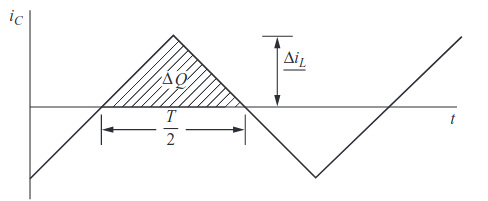
\includegraphics[width=0.8\textwidth]{../images/hart/buck_converter_capacitor_current.png}
    \caption{Corriente por el capacitor de salida}
    \label{fig:buck_converter_capacitor_current}
\end{figure}

La variación de la carga, $\Delta Q$, es el área del triángulo situado por encima del eje de tiempo:

$$ \Delta Q=\frac{1}{2}\left(\frac{T}{2}\right)\left(\frac{\Delta i_{L_x}}{2}\right)=\frac{T\Delta i_{L_x}}{8} $$

Reemplazando:

$$ \Delta V_o=\frac{T\Delta i_{L_x}}{8C} $$

Sustituyendo el valor de la variación de corriente en la bobina cuando el interruptor está abierto, 
se obtiene la tensión de rizado pico a pico en la salida, mostrada en la figura \ref{fig:buck_converter_capacitor_ripple_voltage}.

$$ \Delta V_o=\frac{T}{8C}\frac{V_o}{L}(1-D)T=\frac{V_o(1-D)}{8LCf^2} $$

\begin{figure}[ht]
    \centering
    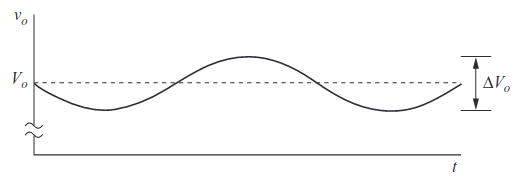
\includegraphics[width=0.8\textwidth]{../images/hart/buck_converter_capacitor_ripple_voltage.png}
    \caption{Tensión de rizado pico a pico a la salida}
    \label{fig:buck_converter_capacitor_ripple_voltage}
\end{figure}

Si el rizado no es muy grande, la suposición de que la salida es constante es razonable, y el
análisis anterior será válido.

En resumen, cuando el interruptor está cerrado, la fuente entrega energía a la carga a través del transformador.
La tensión en el secundario es una forma de onda pulsante. La energía almacenada en
la inductancia magnetizante cuando el interruptor está cerrado es devuelta a la fuente de
entrada a través de un tercer devanado cuando el interruptor está abierto.

En comparación con la topología flyback, el convertidor forward requiere de una carga mínima para evitar un exceso en la tensión de salida. 
Como el transformador no almacena energía, para un mismo nivel de potencia de salida, 
el tamaño del mismo es menor en el convertidor forward que en el flyback. 
Además, la corriente de salida es aproximadamente constante ya que el ripple disminuye notablemente 
debido al agregado del inductor en la salida y al diodo de rueda libre $D_2$.
Por esto mismo, el capacitor de salida puede ser más pequeño. 

\subsubsection{Convertidor Forward Doble Switch}

El convertidor forward se utiliza para potencias de salida de hasta 250W ya que se encuentra limitado 
por los esfuerzos de tensión y corriente a los que se somete el transistor de potencia durante su funcionamiento. 
El convertidor forward de doble switch puede ser utilizado con potencias de hasta 500W.
En la figura \ref{fig:forward_doble_switch} se muestra el esquema de éste último.
A partir de los diodos $D_3$ y $D_4$ en el primario se reduce la tensión de colector en los transistores cuando los mismos 
se encuentran apagados, lo cual permite utilizar transistores de menores prestaciones.

\begin{figure}[H]
    \centering
    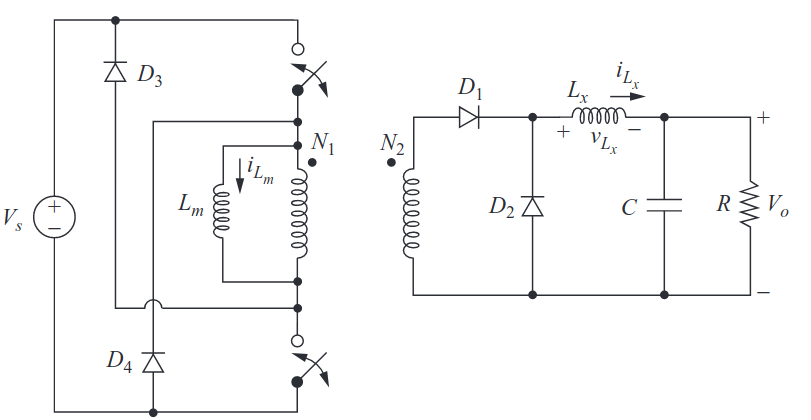
\includegraphics[width=0.8\textwidth]{../images/hart/forward_doble_switch.png}
    \caption{Esquema del convertidor forward de doble switch}
    \label{fig:forward_doble_switch}
\end{figure}

\begin{figure}[H]
    \centering
    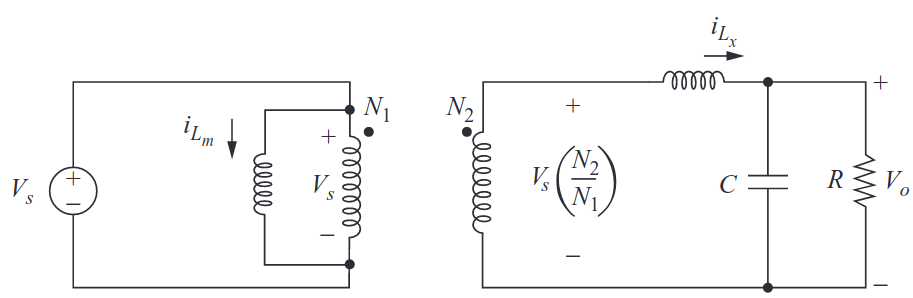
\includegraphics[width=0.8\textwidth]{images/hart/forward_doble_switch_closed.png}
    \caption{Convertidor forward doble switch cuando los interruptores están cerrados}
    \label{fig:forward_doble_switch_closed}
\end{figure}

Los transistores se encienden y se apagan de forma simultánea. 
En la figura \ref{fig:forward_doble_switch_closed} se muestra el circuito equivalente cuando los interruptores están cerrados.  
Cuando los transistores están encendidos, la tensión en el primario del transformador es igual a la tensión de entrada $V_s$. 
En consecuencia, la tensión en el devanado secundario es positiva y la energía se transfiere a la carga. 
Además la corriente que circula por la inductancia magnetizante se incrementa con el tiempo. 

\begin{figure}[H]
    \centering
    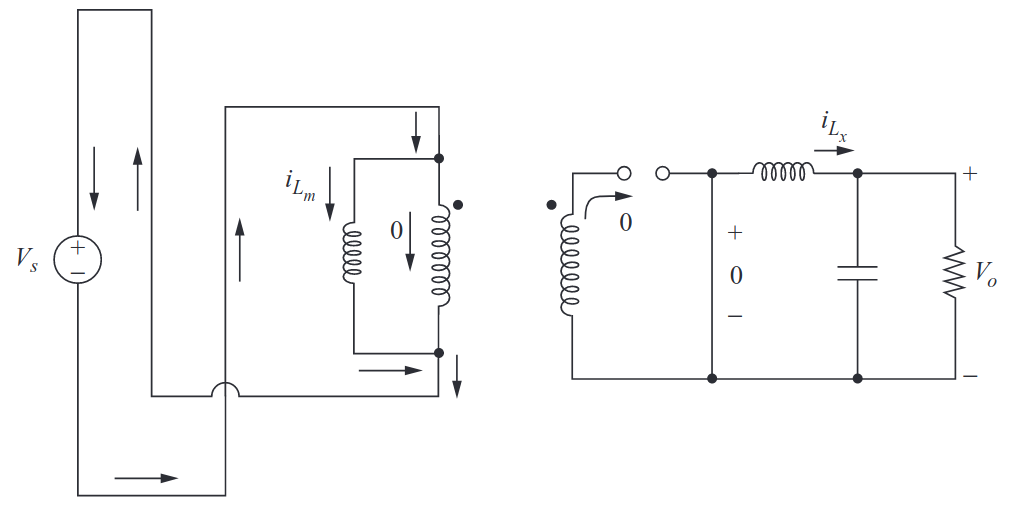
\includegraphics[width=0.8\textwidth]{images/hart/forward_doble_switch_open.png}
    \caption{Convertidor forward doble switch cuando los interruptores están abiertos}
    \label{fig:forward_doble_switch_open}
\end{figure}

En la figura \ref{fig:forward_doble_switch_open} se muestra el circuito equivalente cuando los interruptores están abiertos.  
Cuando los transistores se apagan, el diodo $D_1$ evita que la corriente magnetizante circule por el secundario 
(y por lo tanto también en el primario) del transformador, forzando su camino por los diodos $D_3$ y $D_4$ de regreso a la fuente de entrada.  
Con esto se elimina la necesidad del tercer devanado de desmagnetización, y la tensión en el primario del transformador es $-V_s$, causando un decremento en el tiempo de la corriente magnetizante. 

Si la relación de trabajo de los transistores es menor a 0.5, en cada ciclo el núcleo del transformador se restablece.
La tensión de salida es la misma que en el convertidor forward con un interruptor descrito anteriormente.
La principal ventaja de esta topología es que la tensión de colector en los transistores cuando los mismos se encuentran apagados 
es $V_s$ y no $V_s\left(1+N_1/N_3\right)$ como en el forward de un único switch.

\subsection{Circuito de control}
% El diseño se realizó en bloques según la figura \ref{fig:marco_teorico:control} y puede ser dividido en tres partes:

% \begin{enumerate}
%     \item Compensador y generador PWM
%     \item Selector de modo de funcionamiento
%     \item Controlador para los switches
% \end{enumerate}

% Para la selección de un controlador para los MOSFETs se tuvieron en cuenta algunos parámetros como
% la tensión máxima de entrada, frecuencia de switching y sincronización de las señales,
% pero no se logró hallar un controlador adecuado para esta aplicación.
% El principal motivo fue que los controladores convencionales generan señales alternadas mediante el método de bootstrapping \cite{hart},
% lo cual no sirve para la topología elegida. Esto, combinado con el elevado nivel de tensión en la entrada,
% llevó a la búsqueda de otros métodos de control; por eso, se optó por un controlador con transformador aislante para el MOSFET cuyo source no esta a tierra \cite{gatedrivers}. El diagrama de este driver puede observarse en la figura \ref{fig:driver}.

\subsubsection{Modos de control}

La tensión de salida del convertidor puede ser controlada variando el ciclo de trabajo $D$. 
Para ello, los convertidores funcionan con un circuito de realimentación,
en un control por tensión o corriente, dependiendo de la señal realimentada. 

\begin{figure}[ht]
    \centering
    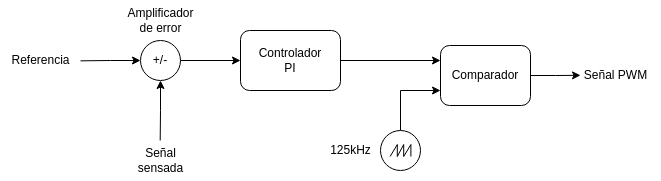
\includegraphics[width=0.8\textwidth]{images/compensador.png}
    \caption{Diagrama de bloques del circuito de control}
    \label{fig:marco_teorico:control}
\end{figure}

\paragraph{Control por tensión}
%COMPLETAR CON LIBRO
En la figura \ref{fig:marco_teorico:control} se muestra un diagrama en bloques del circuito de control.
El circuito de control mide la tensión a la salida del convertidor, la escala a partir de un divisor resistivo y la compara con la tensión deseada.
El amplificador de error es un amplificador operacional que compara la señal de entrada con una referencia y
amplifica la diferencia entre ambas. Su señal de salida es una señal de error, la cual alimenta a un controlador controlador proporcional-integrador (PI).
El mismo está conformado por dos amplificadores operacionales, uno de ellos integra la señal de entrada y el otro la escala.
Las salidas de ambos amplificadores se suman y se obtiene la señal de entrada del comparador.
Éste último compara la señal de entrada con una señal diente de sierra, y en base a esto genera la señal PWM que controla a los transistores.

La frecuencia de switching es definida por la frecuencia de la señal de diente de sierra y se eligió un valor típico de $f=125kHz$.
Como se observa en la figura \ref{fig:pwm-nose}, el tiempo de encendido de la forma de onda PWM inicia cuando se reestablece el generador de dientes de sierra y finaliza cuando su rampa positiva se intersecta con la señal de tensión de error.
Cuando la tensión de salida es inferior al valor nominal, la señal de error generada incrementa su duración y provoca un aumento en el ciclo de trabajo y, en consecuencia, en la tensión de salida. 
En el caso de que la tensión de salida sea superior a la nominal, el proceso es análogo causando una disminución del ciclo de trabajo. 

\begin{figure}[H]
    \centering
    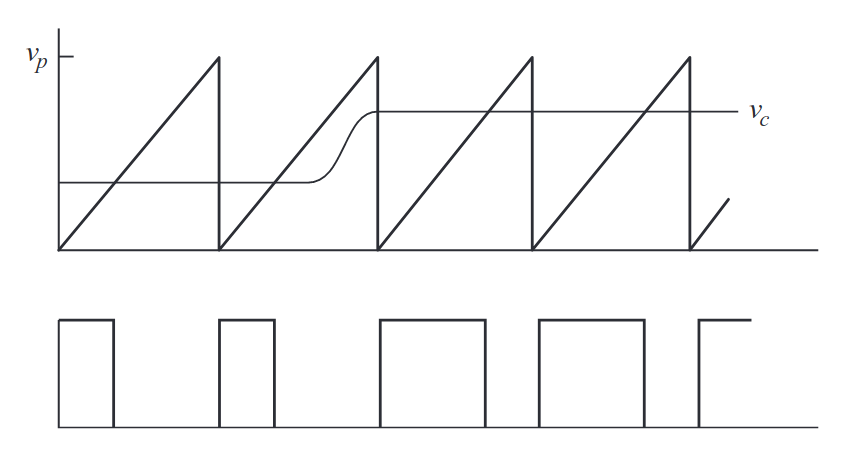
\includegraphics[width=0.8\textwidth]{../images/hart/pwm-info.png}
    \caption{Señales de entrada y de salida del comparador}
    \label{fig:pwm-nose}
\end{figure}
%La dinámica de retroalimentación está determinada por el circuito amplificador de error que consta de Z1 y Z2.

\paragraph{Control por corriente}
La corriente a la salida del convertidor es medida con una resistencia de bajo valor conectada en serie con la carga.
Esta resistencia actúa como un transductor de corriente a tensión.
La señal es muestreada y el resto del proceso es análogo al control por tensión.\\

% Consiste en un lazo interno que muestrea el valor de la corriente primaria y apaga los interruptores tan pronto como la corriente alcanza cierto valor establecido por el lazo de voltaje externo. 
% De esta manera, el control de corriente logra una respuesta más rápida que el modo de voltaje. 
% La forma de onda de corriente primaria actúa como onda de diente de sierra. 
% la tensión análoga a la corriente puede ser proporcionada por una pequeña resistencia o por un transformador de corriente. 
% La figura 13.19a muestra un convertidor flyback controlado por modo de corriente, donde la corriente del interruptor isw se usa como señal portadora. 
% La corriente del interruptor isw produce un voltaje a través de Rs, que se retroalimenta al comparador. 
% El encendido está sincronizado con el pulso del reloj y el apagado está determinado por el instante en que la corriente de entrada es igual al voltaje de error.
% Debido a su capacidad inherente de limitación de corriente máxima, el control de modo de corriente puede mejorar la confiabilidad de los interruptores de alimentación. El rendimiento dinámico se mejora debido al uso de la información actual adicional. El control de modo de corriente reduce efectivamente el sistema a primer orden al obligar a que la corriente del inductor se relacione con el voltaje de salida, logrando así una respuesta más rápida. Las figuras 13.18b–e muestran las formas de onda.

% COMPLETAR CON JUSTIFICACIÓN DE POR QUÉ NO ELEGIMOS CONTROL POR CORRIENTE QUE PARECERÍA SER MEJOR. 

\subsubsection{Selector de modo de funcionamiento}

Permite alternar entre los diferentes modos de carga: precarga, corriente constante y tensión constante. 
En la figura \ref{fig:esquema_selector} se puede observar el esquema de este circuito.

\begin{figure}[H]
    \centering
    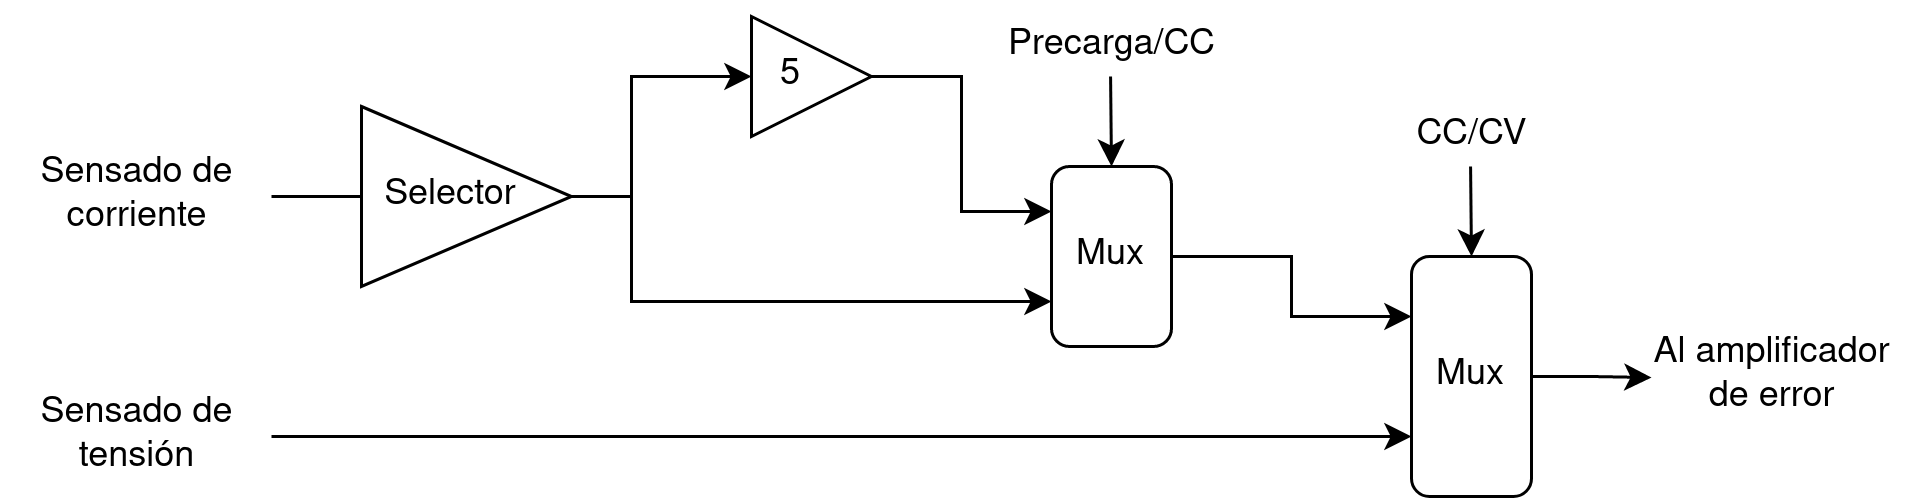
\includegraphics[width=\textwidth]{images/selector.png}
    \caption{Esquema del selector de modo}
    \label{fig:esquema_selector}
\end{figure}

% Un amplificador de ganancia variable actúa como selector de corriente de salida,
% modificando la amplitud de la señal de control de dicha variable.
El amplificador de ganancia variable de la izquierda es el encargado de seleccionar la corriente de salida.
Esto se logra variando la ganancia del operacional.

La selección entre el modo de precarga y el modo de corriente constante se realiza comparando el nivel de tensión de la batería con una señal de referencia.
El modo de precarga se activa una vez que la tensión supera los 30V.

% El bloque de ganancia 5 amplifica la señal de control, ya que la corriente de salida para el modo de precarga es 5 veces inferior a la de la etapa de corriente constante.
%Aumentar la amplitud de la señal de control causará una disminución proporcional de la corriente de salida,
Posterior al selector de corriente, el bloque de ganancia en la bifurcación superior permite tener una señal de control 5 veces mayor para el modo de precarga.
La amplitud de la señal de control es inversamente proporcional a la señal de salida,
por lo que la corriente de salida será 5 veces menor cuando se cierre el lazo por esa rama.

Las señales de tensión y corriente están normalizadas con respecto a sus valores nominales, lo cual permite que el último multiplexor seleccione la señal de mayor amplitud. De esta forma se pueden establecer los límites de tensión y corriente de salida para seguir el perfil de carga deseado.

\subsubsection{Generador PWM}

Por lo general se utilizan circuitos integrados controladores PWM que sólo requieren de unos pocos componentes pasivos adicionales para su funcionamiento. 
Se utilizó el TL494 como generador de señal PWM de frecuencia fija \cite{tl494}. 
Como se observa en la figura \ref{fig:tl494-block-diagram}, internamente presenta 4 componentes principales:
\begin{enumerate}
    \item Un reloj ajustable que permite configurar la frecuencia de conmutación
    \item Dos amplificadores de error para la tensión de salida sensada y la deseada
    \item Un generador de forma de onda de dientes de sierra sincronizado con el reloj
    \item Un comparador para comparar la señal de error de salida con la señal de dientes de sierra
\end{enumerate}
 
\begin{figure}[H]
    \centering
    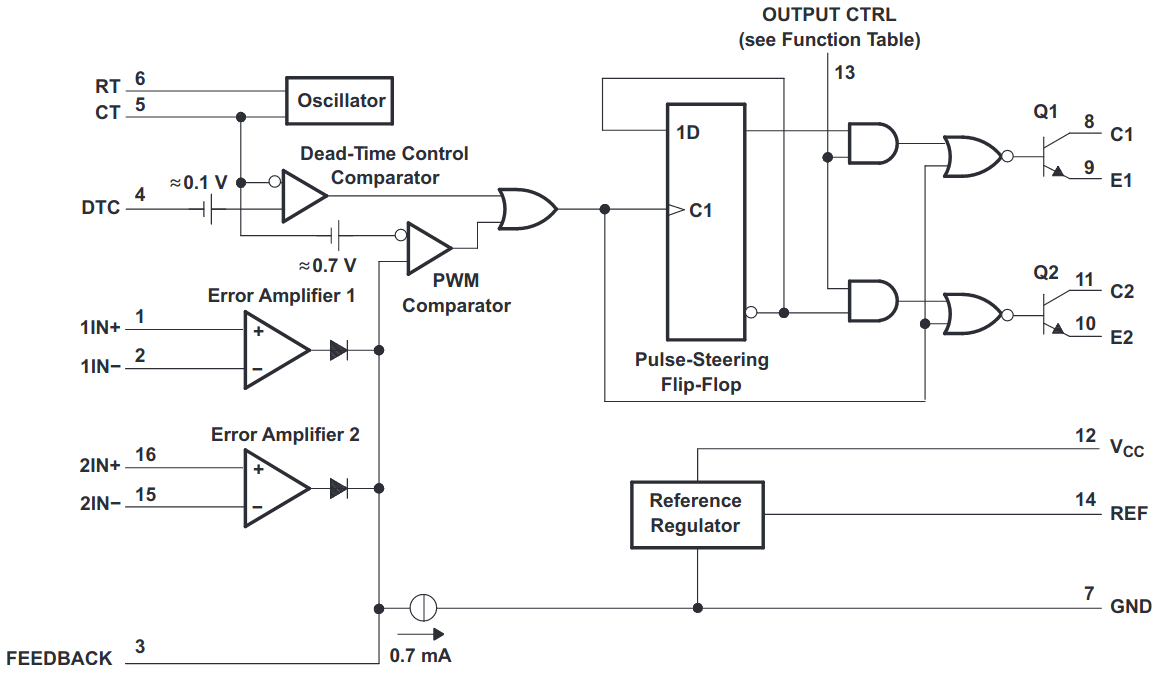
\includegraphics[width=0.8\textwidth]{images/tl494-schematic.png}
    \caption{Diagrama en bloques del TL494}
    \label{fig:tl494-block-diagram}
\end{figure}

El rango de suministro de la tensión de entrada va desde los 7V hasta los 40V. 
Presenta un regulador interno de 5V con precisión del 5\% para la alimentación de sus componentes internos.
Posee dos transistores de salida que pueden trabajar tanto en emisor común como en colector común. 
Un flip-flop de dirección de pulso dirige alternativamente el pulso modulado a cada uno de los dos transistores de salida. 
La corriente de salida máxima de estos transistores es de $250mA$.

Un oscilador interno provee la forma de onda de diente de sierra al comparador PWM. 
Su frecuencia se programa mediante la selección de una resistencia $R_t$ y un capacitor $C_t$. 
El oscilador carga al capacitor con una corriente constante $I_{carga}$ determinada por la resistencia produciendo una rampa de tensión sobre el mismo.

$$ I_{carga}=\frac{3V}{R_t} $$

Cuando la tensión sobre el mismo llega a $3V$, el circuito se descarga y se reinicia el ciclo. 
La frecuencia está definida por la siguiente fórmula:

$$ f=\frac{1}{R_t\times C_t} $$

Según la hoja de datos, los valores recomendados para el filtro RC externo son:

$$ 470pF\leq C_t\leq 10\mu F$$
$$ 1.8k\Omega\leq R_t\leq 500k\Omega $$

Se anticipa que una incorrecta elección de $R_t$ y $C_t$ para el TL494 fuera de los valores recomendados por el fabricante generaba variaciones muy grandes de la frecuencia de conmutación, 
lo cual causaba inestabilidad en la tensión de salida. 
Utilizando valores recomendados para ambos componentes se logró que la frecuencia posea una gran estabilidad.
Para lograr la frecuencia de $f=125kHz$ se eligió un capacitor de $1nF$ y para la resistencia de $8k\Omega$ se ajustó un potenciómetro de $10k\Omega$. 

El comparador permite la modulación de los pulsos de salida, comparando la rampa de tensión sobre el capacitor $C_t$ con cualquiera de las dos señales de control presentes en las salidas de los amplificadores de error.
La etapa de salida se habilita durante el tiempo en el cual la tensión de diente de sierra es mayor que las señales de control de voltaje. 
A medida que aumenta la señal de control, disminuye el tiempo durante el cual la entrada de diente de sierra es mayor, y en consecuencia también decrece la duración del pulso de salida. 
Su tiempo de respuesta es de $400ns$.

El control de tiempo muerto (DTC) permite controlar el ciclo de trabajo. 
Es una entrada de alta impedancia que controla el tiempo de apagado mínimo. Con DTC a tierra, este es del 3\%, pero si se aplica tensión en este puerto se le puede adicionar.
El tiempo muerto se controla linealmente variando su tensión de entrada entre $0$ y $3.3V$, desde su mínimo de 3\% hasta su máximo de 100\% respectivamente. 
% Dos amplificadores de error:
% Presentan alta ganancia y se alimentan mediante su entrada $V_i$. 
% Tensión de MC de entrada: -0.3V a $V_{cc}-2V$

% Output-Control Input:
% Determina el modo de operación de la salida de los transistores. 
% Si está a tierra opera en modo single-ended o modo paralelo donde los pulsos vistos en la salida del DTC son transmitidos por ambos transistores de salida en paralelo.
% Si está a Vref opera en push-pull donde cada transistor de salida está habilitado alternativamente por el flip-flop de dirección de pulsos.

% Transistores de salida:
% El integrado incluye 2 transistores que tienen la posibilidad de ser emisor común o seguidor por emisor. 
% Son capaces de generar hasta $200mA$ de salida. 

% REVISAR SI ES DEL TL494 O ES UNA NOTA AL TUN TUN
% Transformador: permite que no circule corriente continua por su secundario. 

\subsection{Amplificador clase B con transistores complementarios}

La etapa permite acoplar la carga en continua. 
Como se observa en la figura \ref{fig:complementarios}, se compone de un transistor NPN y otro PNP, ambos dispositivos de potencia y no de señal. 
Cada dispositivo de amplificación conduce durante medio ciclo de la señal de entrada, 
excitándolos mediante el ingreso de corriente por su base y lo hacen de forma alternativa. 
En el semiciclo positivo de la señal conduce el NPN y el PNP se corta, y en el semiciclo negativo conduce el PNP y el NPN se corta \cite{Gi}.

Los transistores se alimentan de forma inversa: el NPN requiere de una tensión positiva en su colector y el PNP requiere de una tensión negativa en su colector.
Además, requieren de una tensión $V_{be}$ en sus junturas ya que entre base y emisor existe una juntura PN similar a un diodo. 
Si no se polariza de forma correcta, no circula corriente por su base y en consecuencia tampoco por su colector. 
El transistor NPN conduce corriente en su emisor cuando $V_{be}>0$ mientras que el transistor PNP conduce corriente en su emisor cuando $V_{be}<0$ o $V_{eb}>0$.
Cuando la tensión de entrada en la base de ambos transistores es 0 no conduce ningún transistor, es decir, no existe consumo de corriente ni de potencia. 
% La $V_{ce}$ de ambos transistores va de $V_{cc}$ a 0.

\begin{figure}[H]
    \centering
    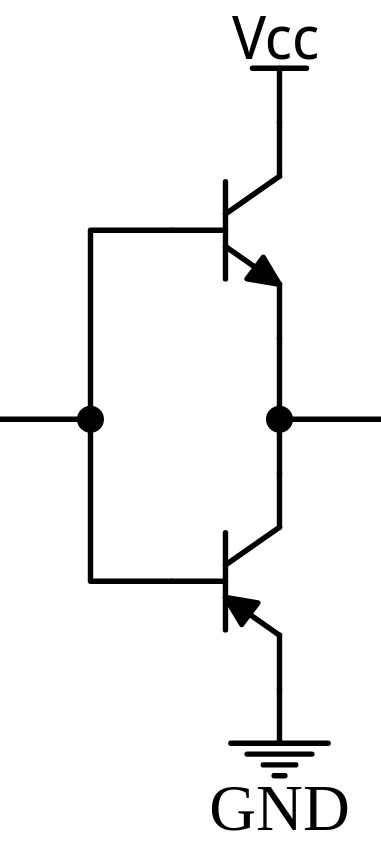
\includegraphics[width=0.2\textwidth]{images/clase-b.png}
    \caption{Amplificador con transistores complementarios}
    \label{fig:complementarios}
\end{figure}

Ambos funcionan como seguidor por emisor o colector común, con su tensión de alimentación en colector, la señal de excitación en la base y la carga conectada al emisor. 
La topología presenta una ganancia de tensión aproximadamente unitaria y una ganancia de corriente $hfe$. 
La corriente que se entrega por la base es $hfe$ veces menor que la que se le entrega a la carga. 
Presenta una impedancia de entrada mucho más alta que su impedancia de salida, la cual se adapta con una carga de baja impedancia. 
Por lo tanto, la etapa amplificadora permite que por la salida circule la misma corriente que requería el convertidor, pero con una corriente de salida del TL494 por colector mucho más baja y menor a la máxima. 

\subsection{Driver}

Para encender los MOSFETs de canal N necesarios en el convertidor se debe aplicar una tensión positiva entre \textit{gate} y \textit{source}. 
Debido a la topología elegida, se requiere un driver para controlar el MOSFET cuyo terminal de \textit{source} no está a tierra.
Existen 2 posibles configuraciones para un transistor según su posición respecto a la carga:

\paragraph{Lado bajo} Utiliza comúnmente el MOSFET de canal N. 
El terminal \textit{source} está a tierra y la carga se encuentra entre la alimentación y el terminal \textit{drain}. 

\paragraph{Lado alto} Utiliza comúnmente el MOSFET de canal P. 
El terminal \textit{drain} se encuentra conectado a la alimentación y el terminal \textit{source} a la carga.\\

% INSERTAR FIGURA DE YCIRCUIT YA SUBIDA
\begin{figure}[H]
    \centering
    \centering
    \begin{minipage}{0.45\textwidth}
        \centering
        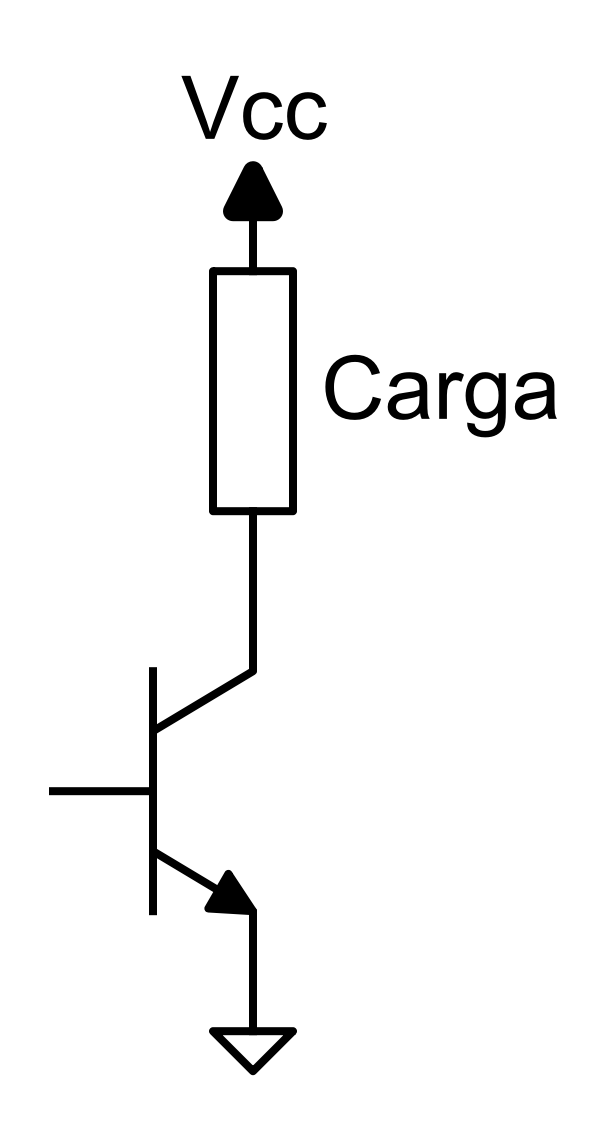
\includegraphics[width=0.5\textwidth]{images/low_high_side/Low_Side.png}
    \end{minipage}
    \begin{minipage}{0.45\textwidth}
        \centering
        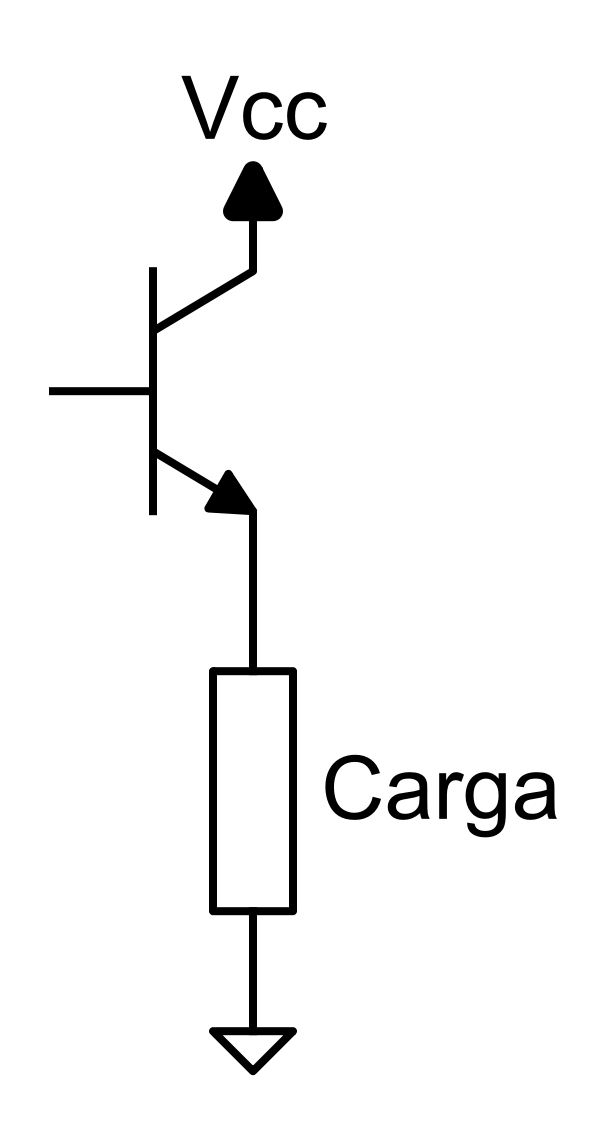
\includegraphics[width=0.5\textwidth]{images/low_high_side/High_Side.png}
    \end{minipage}
    \caption{A la izquierda, un transistor de lado bajo. A la derecha, uno de lado alto.}
    \label{fig:high_side}
\end{figure}

Para controlar MOSFETs de lado alto se puede utilizar un circuito integrado o un transformador. 
Los circuitos integrados, si bien son más pequeños y ocupan menor espacio en las placas, 
poseen tiempos significativos de encendido y apagado. 
El transformador es de un tamaño mucho mayor, requiere de un diseño apropiado y de componentes adicionales,
pero sus tiempos de encendido y apagado son despreciables y permite operar con diferencias de tensión más elevadas.
En base a ello, se optó por implementar un transformador como driver para el MOSFET de lado alto \cite{gatedrivers}. 

Los transformadores poseen al menos 2 bobinados acoplados magnéticamente, 
lo cual permite generar aislación entre el circuito primario y secundario. 
La relación de vueltas entre los mismos permite modificar la tensión de salida obtenida. 
Los transformadores manejan muy poca potencia promedio, pero entregan altos picos de corriente en el encendido y apagado.

Si bien el transformador ideal no almacena energía, los transformadores reales 
almacenan una pequeña cantidad de energía entre los bobinados y el posible entrehierro. 
Esto se representa mediante una inductancia magnetizante en paralelo al bobinado del primario. 
Una pequeña inductancia disminuye los retrasos de tiempo y minimiza la energía almacenada permitiendo aumentar la eficiencia. 

Para cumplir con la ley de Faraday, la tensión en la bobina del transformador debe ser nula en una parte del período, 
por lo cual cualquier pequeña señal de continua puede hacer saturar al núcleo. 
La saturación limita el producto volt-segundo aplicado a través de los devanados. 
Su valor máximo se da en la peor condición de funcionamiento, con el ciclo de trabajo máximo y la máxima tensión de entrada de forma simultánea. 

Como el convertidor forward trabaja sólo en el primer cuadrante del plano B-H, una gran parte del período de switching debe reservarse para restaurar el núcleo de la potencia del transformador \cite{hart_espanol}.
Esto limita la relación de trabajo del transformador, pero no suele ser un problema ya que 
el transformador debe estar acoplado a corriente alterna y por lo tanto funciona con magnetización bidireccional.

\begin{figure}[H]
    \centering
    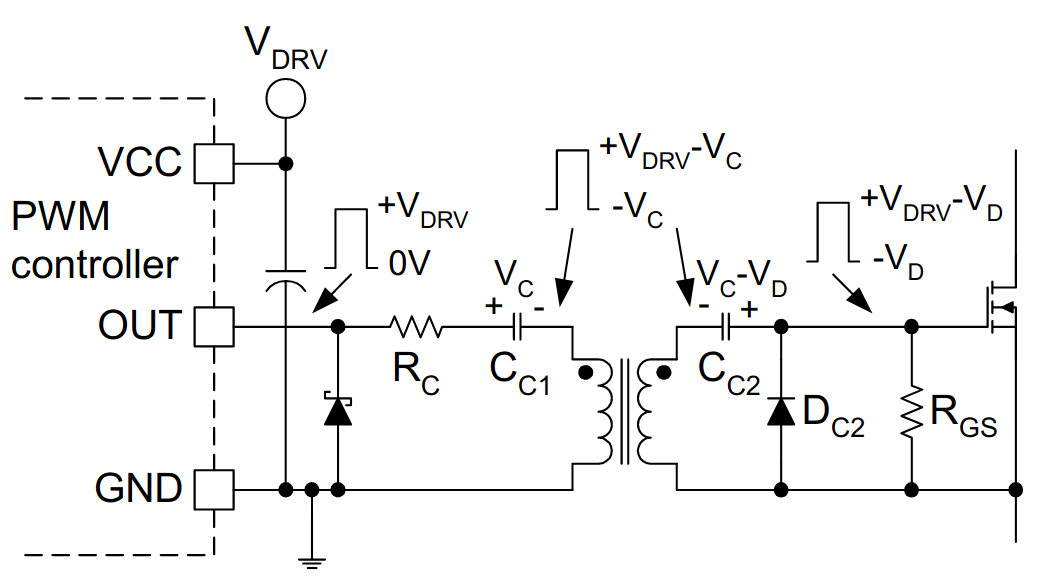
\includegraphics[width=\textwidth]{images/esquema_driver.png}
    \caption{Esquema del controlador del MOSFET de lado alto}
    \label{fig:driver}
\end{figure}

La figura \ref{fig:driver} muestra el circuito básico del driver mediante un transformador.
A continuación se detalla información relevante de cada componente: 

\paragraph{Entrada single-ended} 

Este driver en particular está diseñado para convertir la salida de un extremo de un controlador PWM a una señal de doble extremo. % Traduccion de mierda

\paragraph{Capacitor de acoplamiento $C_{C_1}$}

Para evitar la componente continua se coloca un capacitor de acoplamiento en serie con el bobinado primario, 
evitando la saturación del núcleo. La tensión sobre el mismo resulta: 

$$ V_{cc_1}=D\times V_{drv} $$

En base al máximo ripple de tensión permitido y la carga que atraviesa al capacitor de acoplamiento en estado estacionario:

$$ C_{C_1}=\frac{Q_G}{\Delta V_{C_1}}+\frac{(V_{drv}-V_{dc2,fw})D}{\Delta V_{C_1}R_{gs}f_{drv}}+\frac{V_{drv}(D^2-D^3)}{\Delta V_{C_1}\times4\times L_mf_{drv}^2} $$

Para este capacitor, el ripple tiene una componente relacionada a la carga del MOSFET, 
otra relacionada con la corriente que pasa por la resistencia entre \textit{gate} y \textit{source} 
y una última componente relacionada a la corriente de la inductancia magnetizante. 
La capacidad es máxima para un ciclo de trabajo determinado definido por los parámetros de diseño 
y los valores de los componentes, la cual se obtiene derivando a la expresión en función del ciclo. 

La constante de tiempo de la tensión en el capacitor de acoplamiento resulta:

$$ \tau=R_{gs}C_{C_1} $$

La tensión a través del capacitor de acoplamiento se incrementa de forma proporcional al pulso. 
La tensión negativa durante el tiempo que está apagado aumenta y la tensión positiva durante el tiempo que está encendido disminuye. 
Por lo tanto, para pulsos anchos del ciclo de trabajo, se requieren de componentes adicionales 
en el secundario del transformador para proveer de la tensión correcta al \textit{gate}. 

%INSERTAR FORMA DE ONDA SOBRE EL CAPACITOR (SE SACA DEL ESQUEMÁTICO DADO)

\paragraph{Resistencia de amortiguamiento $R_C$}

Cambios repentinos en el ciclo de trabajo excitan a la red LC compuesta por el capacitor de acoplamiento 
y la inductancia magnetizante, provocando resonancias indeseadas en la tensión sobre el capacitor. 
Esta resistencia de bajo valor en serie con el capacitor de acoplamiento permite amortiguar las resonancias. 
Su valor puede calcularse a partir de la siguiente fórmula:

$$ R_c\geq2\times\sqrt{\frac{L_m}{C_{C_1}}} $$

Si la resistencia es muy grande, genera una sobre amortiguación que limita la corriente que ingresa al terminal \textit{gate} y disminuye la frecuencia de switching. 
Si la resistencia es muy chica, las resonancias provocadas generan una tensión entre \textit{gate} y \textit{source} muy elevada.

\paragraph{Transformador}

Su función es transmitir el pulso de accionamiento de puerta referenciado a tierra a través de grandes diferencias de potencial para adaptarse a las implementaciones de accionamiento flotante. 
Para hacerlo maneja muy poca potencia pero requiere de elevados picos de corriente. 
Está controlado por un ancho de pulso variable y de amplitud constante,
acoplado en alterna y la inductancia de magnetización ve un pulso de amplitud variable.
Operan en el primer y tercer cuadrante del plano B-H.

\paragraph{Resistencia de carga entre \textit{gate} y \textit{source} $R_{gs}$}

Es una resistencia de pull down que pone a tierra el terminal \textit{gate} al alimentar el circuito, manteniendo al MOSFET apagado durante el inicio. 
Además le provee de un camino para la corriente que circula por el capacitor de acoplamiento, 
permitiendo establecer la tensión necesaria sobre el mismo y que en cada ciclo de switching 
la misma carga del \textit{gate} sea entregada y removida a través del capacitor. 

\paragraph{Diodo Schottky}

Debido a la componente de corriente de la inductancia magnetizante, la salida debe manejar corriente de forma bidireccional. 
El mismo puede evitarse aumentando la componente de corriente resistiva para contrarrestar a la componente de la inductancia magnetizante. 

\paragraph{Capacitor de acoplamiento $C_{C_2}$}

Junto al diodo Schottky permite restaurar a los niveles originales de tensión. 
El agregado opcional de un diodo zener en serie permite incrementar aún más la tensión negativa durante el apagado. 

En base al máximo ripple de tensión permitido y la carga que atraviesa al capacitor de acoplamiento en estado estacionario:

$$ C_{C_2}=\frac{Q_G}{\Delta V_{C_2}}+\frac{(V_{drv}-V_{dc2,fw})D_{max}}{\Delta V_{C_2}R_{gs}f_{drv}} $$

Para este capacitor, el ripple tiene una componente relacionada a la carga del MOSFET 
y otra relacionada con la corriente que pasa por la resistencia entre \textit{gate} y \textit{source}. 
La capacidad es máxima cuando el ciclo de trabajo es máximo. 

\paragraph{Diodo clamp}

%Evita sobre tensiones. <<< Esto era así? No evitaba tension negativa a la salida?
Mantiene la tensión entre \textit{gate} y \textit{source} por arriba de $-V_\gamma$.\\

\subsection{Snubber} \label{subsec:oscilaciones}

Un circuito snubber o de amortiguación es una red RC que permite eliminar ruido de alta frecuencia que existe en los nodos de los transistores.
Hasta ahora se ha analizado el convertidor forward sin tener en cuenta los elementos parásitos asociados a cada componente. 
Algunos ejemplos de estos son la resistencia serie equivalente e inductancia serie equivalente de los capacitores, 
la capacidad parásita de los transistores o la resistencia e inductancia parásita de las conexiones realizadas. 
La energía acumulada en las inductancias parásitas mientras los transistores conmutan provoca una resonancia con el capacitor de filtrado en la entrada. 
La red snubber conforma un camino de baja impedancia para el drenaje de esta energía \cite{snubber}. 
Valores pequeños de estos elementos parásitos generan resonancias del orden de los MHz. 

\subsubsection{Funcionamiento}

La energía acumulada en las inductancias parásitas mientras los transistores están encendidos se almacena como energía electroestática en el capacitor de la red snubber $C_{snb}$. 
Cuando los transistores conducen, su tensión se eleva hasta $V_{in}$ y la energía almacenada en el capacitor resulta: 

$$ E=0.5\times C_{snb}V_{in}^{2} $$

La carga eléctrica del capacitor luego de su carga es:

$$ Q=C_{snb}V_{in} $$

La potencia suministrada por la fuente de entrada en cada ciclo es:

$$ V_{in}Q=C_{snb}V_{in}^{2} $$

Las pérdidas en la resistencia $R_{sbn}$ resultan:

$$ P_{R_{snb}}=C_{snb}V_{in}^{2}f_{sw} $$

Durante la carga, mitad de esta potencia se consume en la resistencia $R_{snb}$ por efecto Joule y la otra mitad se almacena en el capacitor $C_{snb}$. 
Cuando los transistores no conducen, su tensión disminuye hasta $0V$, toda la energía almacenada se descarga y es consumida en la resistencia de amortiguamiento $R_{snb}$.
Cuando se descarga, mitad de la energía almacenada se convierte en calor en la resistencia $R_{snb}$. 
El análisis supone que el tiempo de carga y descarga es mucho más grande que la constante de tiempo RC. 
El procedimiento para el cálculo de los componentes se describirá detalladamente en la sección de diseño.